\documentclass[11pt, a4paper]{article}
% ══════════════════════════════════════════════════════════════
% Preâmbulo compartilhado pelos documentos da P2
% Reaproveita o estilo de docs/documento-unificado.tex
% ══════════════════════════════════════════════════════════════

\usepackage[utf8]{inputenc}
\usepackage[T1]{fontenc}
\usepackage[brazil]{babel}

\usepackage[top=2.5cm, bottom=2.5cm, left=3cm, right=2cm]{geometry}
\usepackage{setspace}
\onehalfspacing
\setlength{\parindent}{0pt}
\setlength{\parskip}{6pt}

\usepackage{lmodern}
\usepackage{microtype}
\usepackage{amssymb}
\usepackage{amsmath}
\usepackage{pifont}
\newcommand{\cmark}{\ding{51}}
\newcommand{\xmark}{\ding{55}}

\usepackage[table,dvipsnames]{xcolor}
\definecolor{accent}{HTML}{2C7A4B}
\definecolor{accentdim}{HTML}{1E5934}
\definecolor{accentlight}{HTML}{E8F4ED}
\definecolor{tabheader}{HTML}{2C3E50}
\definecolor{tabrow}{HTML}{F5F6FA}
\definecolor{linkblue}{HTML}{2980B9}
\definecolor{codebg}{HTML}{F5F5F5}
\definecolor{codeborder}{HTML}{D0D0D0}
\definecolor{ndvilow}{HTML}{8B4513}
\definecolor{ndvimid}{HTML}{DAA520}
\definecolor{ndvihigh}{HTML}{006400}
\definecolor{warnyellow}{HTML}{F39C12}
\definecolor{successgreen}{HTML}{27AE60}
\definecolor{errorred}{HTML}{E74C3C}

\usepackage{booktabs}
\usepackage{tabularx}
\usepackage{multirow}
\usepackage{makecell}
\usepackage{float}
\usepackage{graphicx}
\usepackage{caption}
\usepackage{array}

\usepackage{enumitem}
\setlist[itemize]{itemsep=2pt, parsep=0pt, topsep=4pt, leftmargin=*}
\setlist[enumerate]{itemsep=2pt, parsep=0pt, topsep=4pt, leftmargin=*}

\usepackage[colorlinks=true, linkcolor=linkblue, urlcolor=linkblue, citecolor=linkblue]{hyperref}

\usepackage{fancyhdr}
\pagestyle{fancy}
\fancyhf{}
\fancyhead[L]{\small\textcolor{gray}{EasyGis}}
\fancyhead[R]{\small\textcolor{gray}{P2 — Gerência e Manutenção de Software · Prof.\ Mauro · 2026.1}}
\fancyfoot[C]{\thepage}
\renewcommand{\headrulewidth}{0.4pt}

\usepackage{titlesec}
\titleformat{\section}
  {\Large\bfseries\color{accentdim}}
  {\thesection.}{0.5em}{}
\titleformat{\subsection}
  {\large\bfseries\color{accent}}
  {\thesubsection}{0.5em}{}
\titleformat{\subsubsection}
  {\normalsize\bfseries}
  {\thesubsubsection}{0.5em}{}

% Listings (código)
\usepackage{listings}
\lstdefinestyle{shellstyle}{
  basicstyle=\ttfamily\small,
  backgroundcolor=\color{codebg},
  frame=single,
  rulecolor=\color{codeborder},
  framesep=4pt,
  xleftmargin=8pt,
  xrightmargin=4pt,
  breaklines=true,
  showstringspaces=false,
  keepspaces=true,
  literate={─}{{-}}1 {├}{{|}}1 {│}{{|}}1 {└}{{`}}1
}
\lstdefinestyle{pythonstyle}{
  basicstyle=\ttfamily\footnotesize,
  language=Python,
  backgroundcolor=\color{codebg},
  frame=single,
  rulecolor=\color{codeborder},
  framesep=4pt,
  xleftmargin=8pt,
  xrightmargin=4pt,
  breaklines=true,
  keywordstyle=\color{accent}\bfseries,
  stringstyle=\color{ndvimid},
  commentstyle=\color{gray}\itshape,
  showstringspaces=false,
  keepspaces=true
}
\lstset{style=shellstyle}

% Caixas para código inline
\newcommand{\code}[1]{\texttt{\colorbox{codebg}{\strut#1}}}

% Caixas de destaque
\usepackage{tcolorbox}
\tcbuselibrary{skins, breakable}

\newtcolorbox{infobox}[1][]{%
  colback=accentlight, colframe=accent,
  boxrule=0.6pt, arc=2pt,
  left=8pt, right=8pt, top=4pt, bottom=4pt,
  fonttitle=\bfseries, breakable, #1
}

\newtcolorbox{warnbox}[1][]{%
  colback=yellow!8, colframe=warnyellow,
  boxrule=0.6pt, arc=2pt,
  left=8pt, right=8pt, top=4pt, bottom=4pt,
  breakable, #1
}

\newtcolorbox{successbox}[1][]{%
  colback=green!4, colframe=successgreen,
  boxrule=0.6pt, arc=2pt,
  left=8pt, right=8pt, top=4pt, bottom=4pt,
  breakable, #1
}


\title{%
  \vspace{-1.5cm}
  {\Huge\bfseries\color{accentdim} Manual do Usuário}\\[8pt]
  {\Large\bfseries ICEV Remote Sensing Software}\\[18pt]
  {\normalsize\itshape Plataforma de Sensoriamento Remoto para Agricultura de Precisão}
}
\author{Equipe ICEV Remote Sensing}
\date{Versão 1.0 --- Maio de 2026}

\begin{document}
\maketitle
\thispagestyle{empty}

\begin{infobox}[title={Para quem é este manual}]
Este manual é destinado a \textbf{produtores rurais, agrônomos, pesquisadores e estudantes}.\\
\textit{Não é necessário conhecimento técnico em programação} para usar o sistema.
\end{infobox}

\vfill
\begin{center}
\small\textit{Instituto de Ensino Superior --- ICEV}\\
\small\textit{Teresina, PI, Brasil}
\end{center}
\newpage

\tableofcontents
\newpage

% ══════════════════════════════════════════════════════════════
\section{O que este sistema faz?}
% ══════════════════════════════════════════════════════════════

O \textbf{ICEV Remote Sensing Software} é uma plataforma web que mostra como está a \textbf{saúde da sua plantação} usando imagens de satélite gratuitas (Sentinel-2 / ESA Copernicus).

Em poucos cliques, você:

\begin{enumerate}
  \item \textbf{Vê o seu talhão} (área agrícola) sobre uma imagem de satélite.
  \item Calcula \textbf{índices de vegetação} (NDVI, EVI, etc.) que mostram, em cores, onde a plantação está saudável e onde precisa de atenção.
  \item Pode \textbf{classificar} o talhão em zonas (alto, médio, baixo vigor) e ver quantos hectares cada zona ocupa.
  \item Visualiza tudo em um \textbf{mapa interativo} ou em \textbf{3D}.
\end{enumerate}

\begin{infobox}
\textbf{Em uma frase:} \textcolor{ndvilow}{\textbf{vermelho/marrom}} = vegetação fraca; \textcolor{ndvimid}{\textbf{amarelo}} = razoável; \textcolor{ndvihigh}{\textbf{verde}} = saudável.
\end{infobox}

% ══════════════════════════════════════════════════════════════
\section{Antes de começar}
% ══════════════════════════════════════════════════════════════

Você precisa que \textbf{alguém com conhecimento técnico} tenha feito a instalação inicial uma única vez. Veja o \texttt{README.md} para isso. Depois disso, basta abrir o sistema e usar.

\subsection{Para abrir o sistema (após a instalação)}

\begin{enumerate}
  \item Abrir um terminal e rodar o backend:
\begin{lstlisting}[style=shellstyle]
./run_api.sh
\end{lstlisting}
  \item Em outro terminal, rodar o frontend:
\begin{lstlisting}[style=shellstyle]
cd web && npm run dev
\end{lstlisting}
  \item Abrir o navegador em \url{http://localhost:3000}
\end{enumerate}

Se algo der errado, peça ajuda ao administrador. Se aparecer ``Frontend OK'' e o mapa carregar, pode usar.

% ══════════════════════════════════════════════════════════════
\section{Tela Inicial --- o que cada coisa faz}
% ══════════════════════════════════════════════════════════════

\begin{figure}[H]
\centering
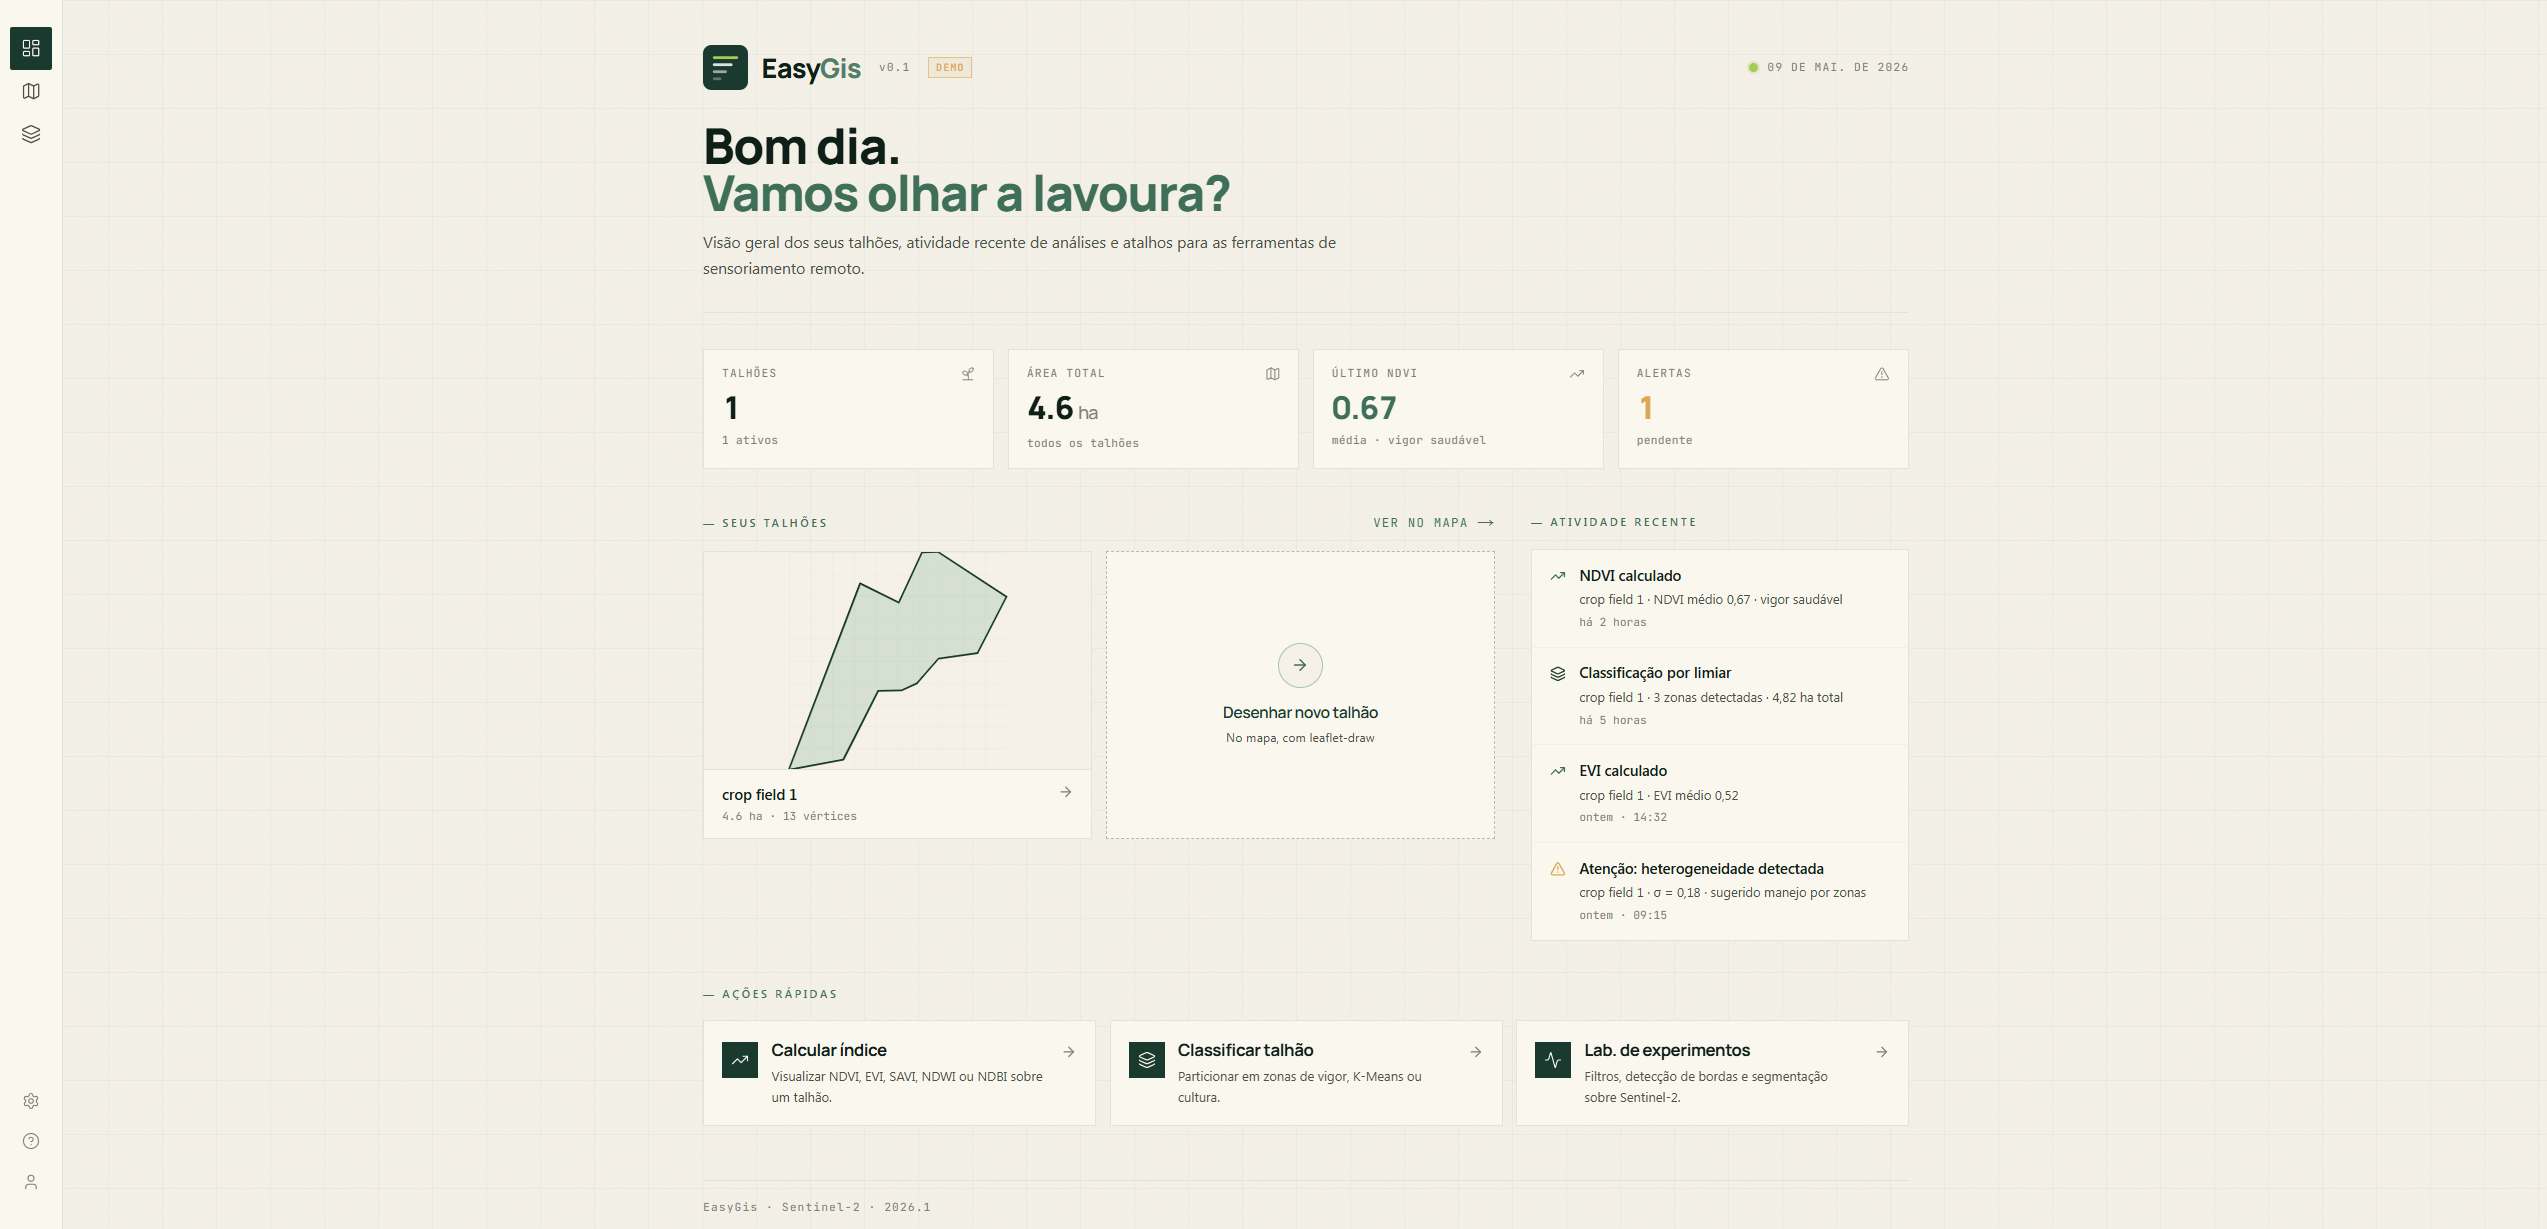
\includegraphics[width=\textwidth]{screenshots/MAN-01_home}
\caption{Tela inicial do sistema --- visão geral com talhões disponíveis e ações rápidas.}
\end{figure}

\renewcommand{\arraystretch}{1.3}
\begin{table}[H]
\centering
\small
\rowcolors{2}{tabrow}{white}
\begin{tabularx}{\textwidth}{@{}lll@{}}
\toprule
\rowcolor{tabheader}\textcolor{white}{\textbf{Onde}} & \textcolor{white}{\textbf{O que é}} & \textcolor{white}{\textbf{Para que serve}}\\
\midrule
Aba ``Analytics'' & Análise rápida & Dia a dia: vê NDVI/EVI do talhão\\
Aba ``Research'' & Pesquisa avançada & Comparar bandas e experimentos\\
Talhão (dropdown) & Lista das suas áreas & Escolha qual área quer analisar\\
Índice (dropdown) & Tipo de análise & NDVI = saúde; EVI = idem corrigido; RGB = foto colorida\\
Botão ``Calcular'' & Roda a análise & Pode demorar 5--30 segundos\\
Mapa & Imagem do satélite & Resultado aparece sobreposto\\
Stats & Números do índice & Mínimo, máximo, média da área\\
Histograma & Gráfico de distribuição & Mostra se o talhão está homogêneo ou desigual\\
Botão 3D & Liga visualização 3D & Vê o índice como ``relevo''\\
\bottomrule
\end{tabularx}
\end{table}

% ══════════════════════════════════════════════════════════════
\section{Como fazer um NDVI em 4 passos}
% ══════════════════════════════════════════════════════════════

\begin{infobox}
\textbf{NDVI = Normalized Difference Vegetation Index.} É o índice mais usado para ver saúde da plantação. Vai de \textbf{$-1$} (água, areia) a \textbf{$+1$} (vegetação muito densa e saudável).
\end{infobox}

\begin{enumerate}
  \item \textbf{Abrir} \url{http://localhost:3000}
  \item No painel lateral esquerdo, clique no dropdown ``Talhão'' e escolha o seu (ex.: \texttt{crop field 1}). O mapa centraliza na área.
\end{enumerate}

\begin{figure}[H]
\centering
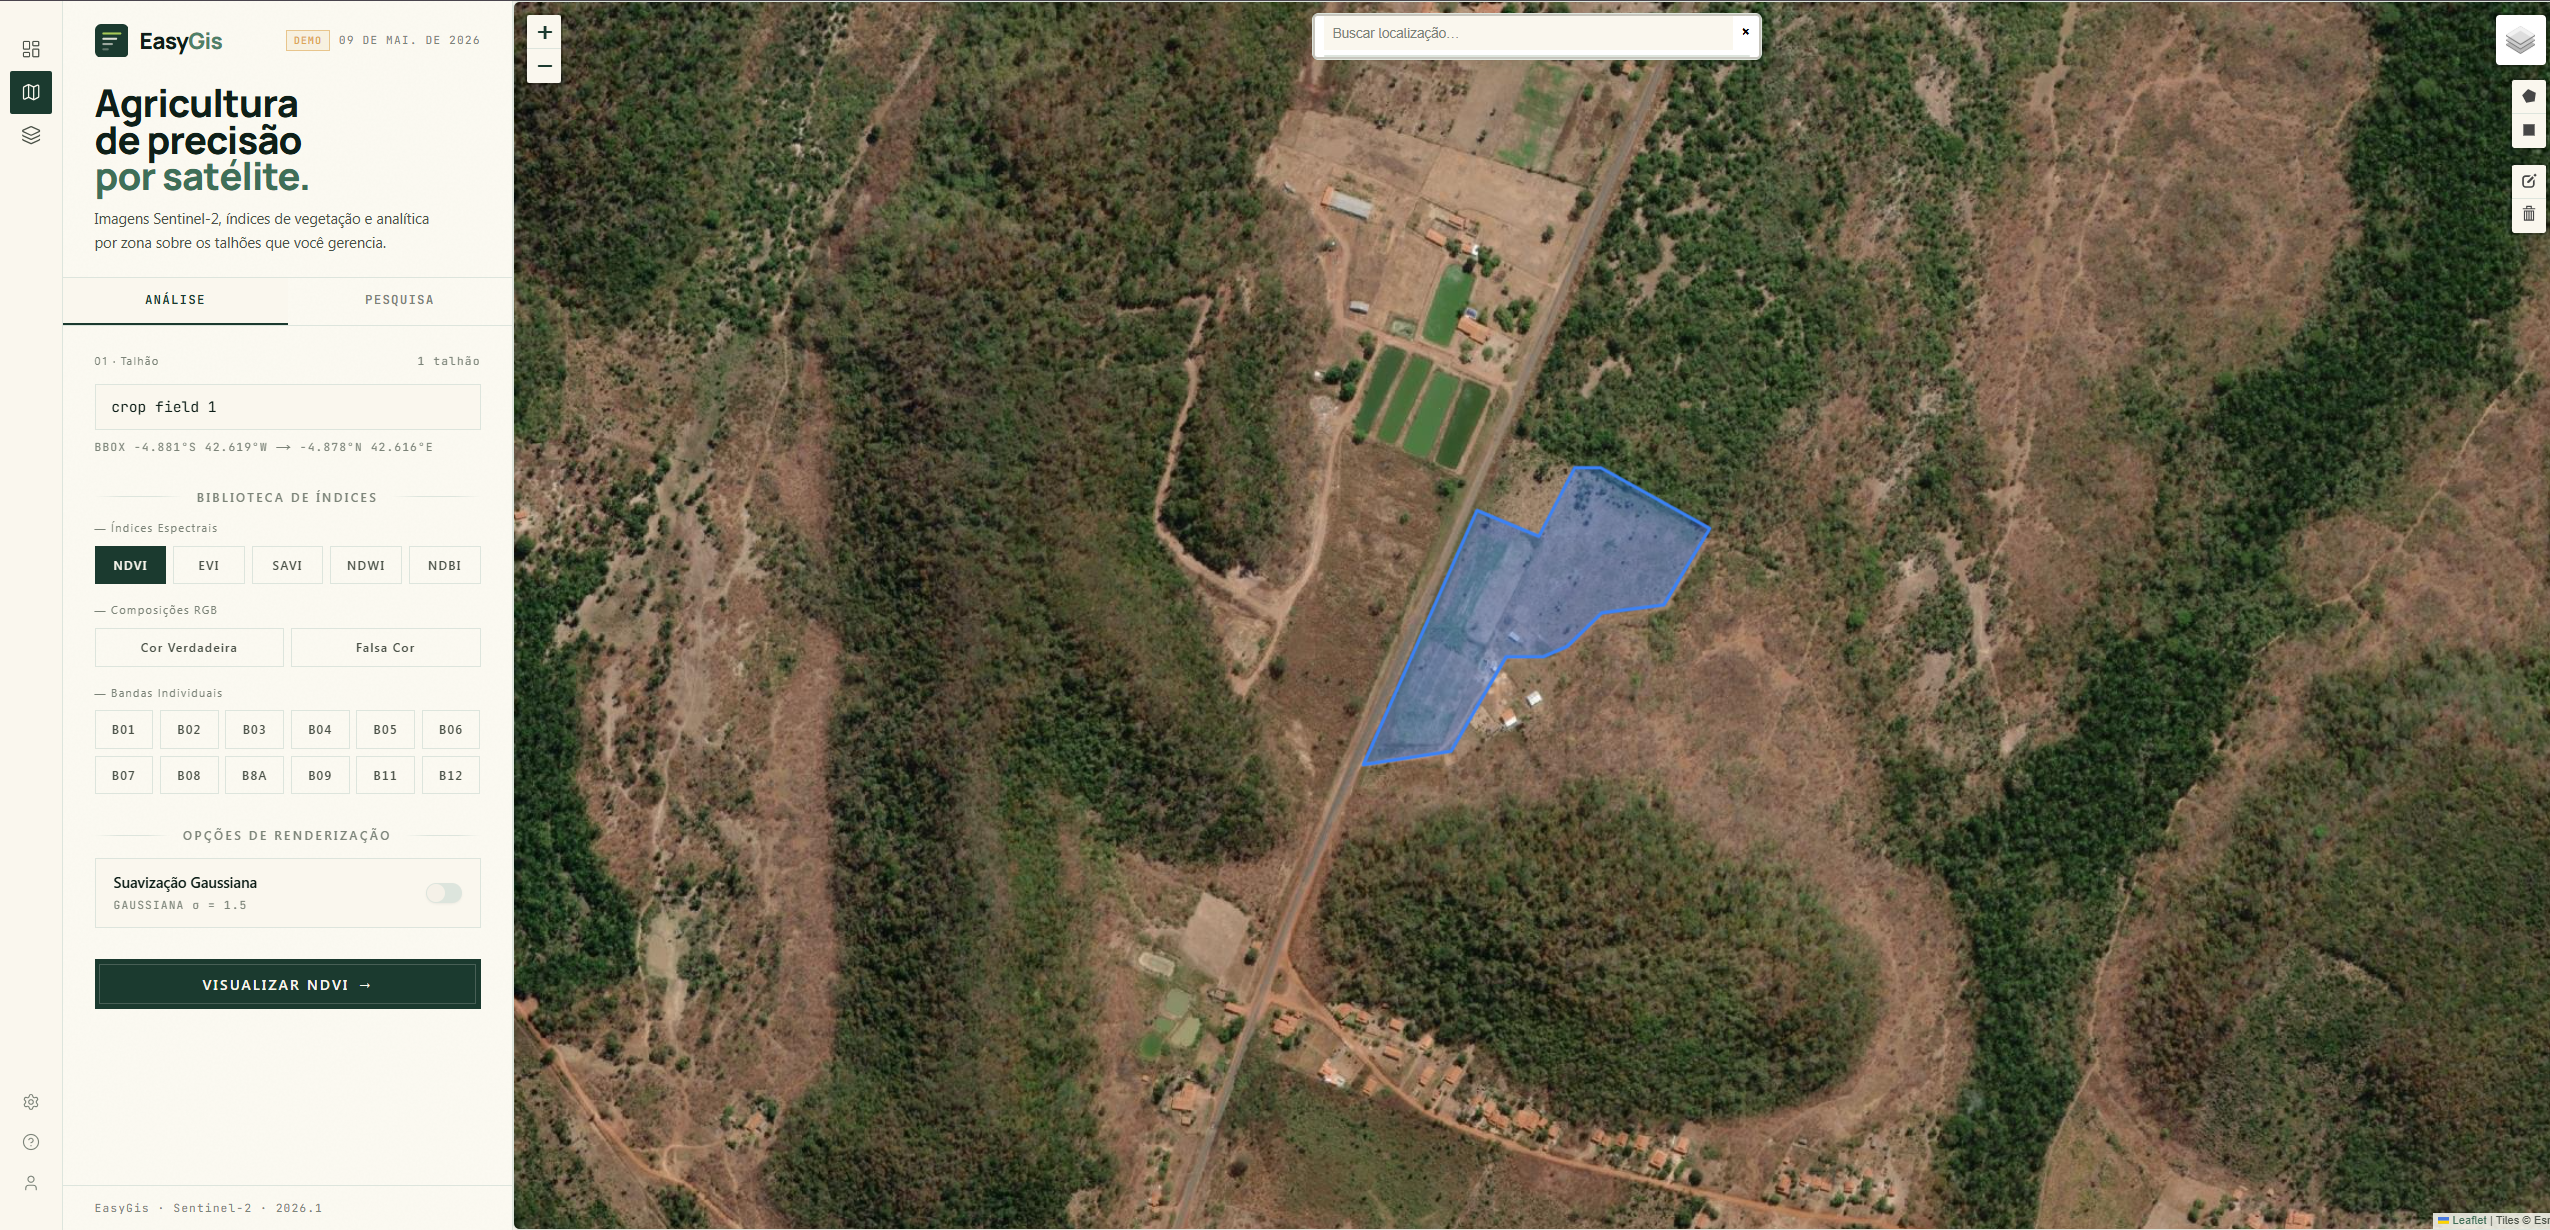
\includegraphics[width=\textwidth]{screenshots/MAN-02_dropdown-talhao}
\caption{Selecionando o talhão no dropdown lateral --- o mapa centraliza automaticamente na área escolhida.}
\end{figure}

\begin{enumerate}\setcounter{enumi}{2}
  \item No dropdown ``Índice'', escolha \texttt{NDVI}. Clique em \textbf{Calcular}.
  \item Aguarde o resultado (5--30 segundos). Quando ficar pronto, você verá:
  \begin{itemize}
    \item Uma camada colorida sobre o talhão (\textcolor{ndvilow}{marrom} = baixo, \textcolor{ndvimid}{amarelo} = médio, \textcolor{ndvihigh}{verde} = alto)
    \item Uma legenda no canto inferior com a escala de cores
    \item As estatísticas no painel lateral (média, máximo, mínimo)
    \item Um histograma mostrando a distribuição
  \end{itemize}
\end{enumerate}

\begin{figure}[H]
\centering
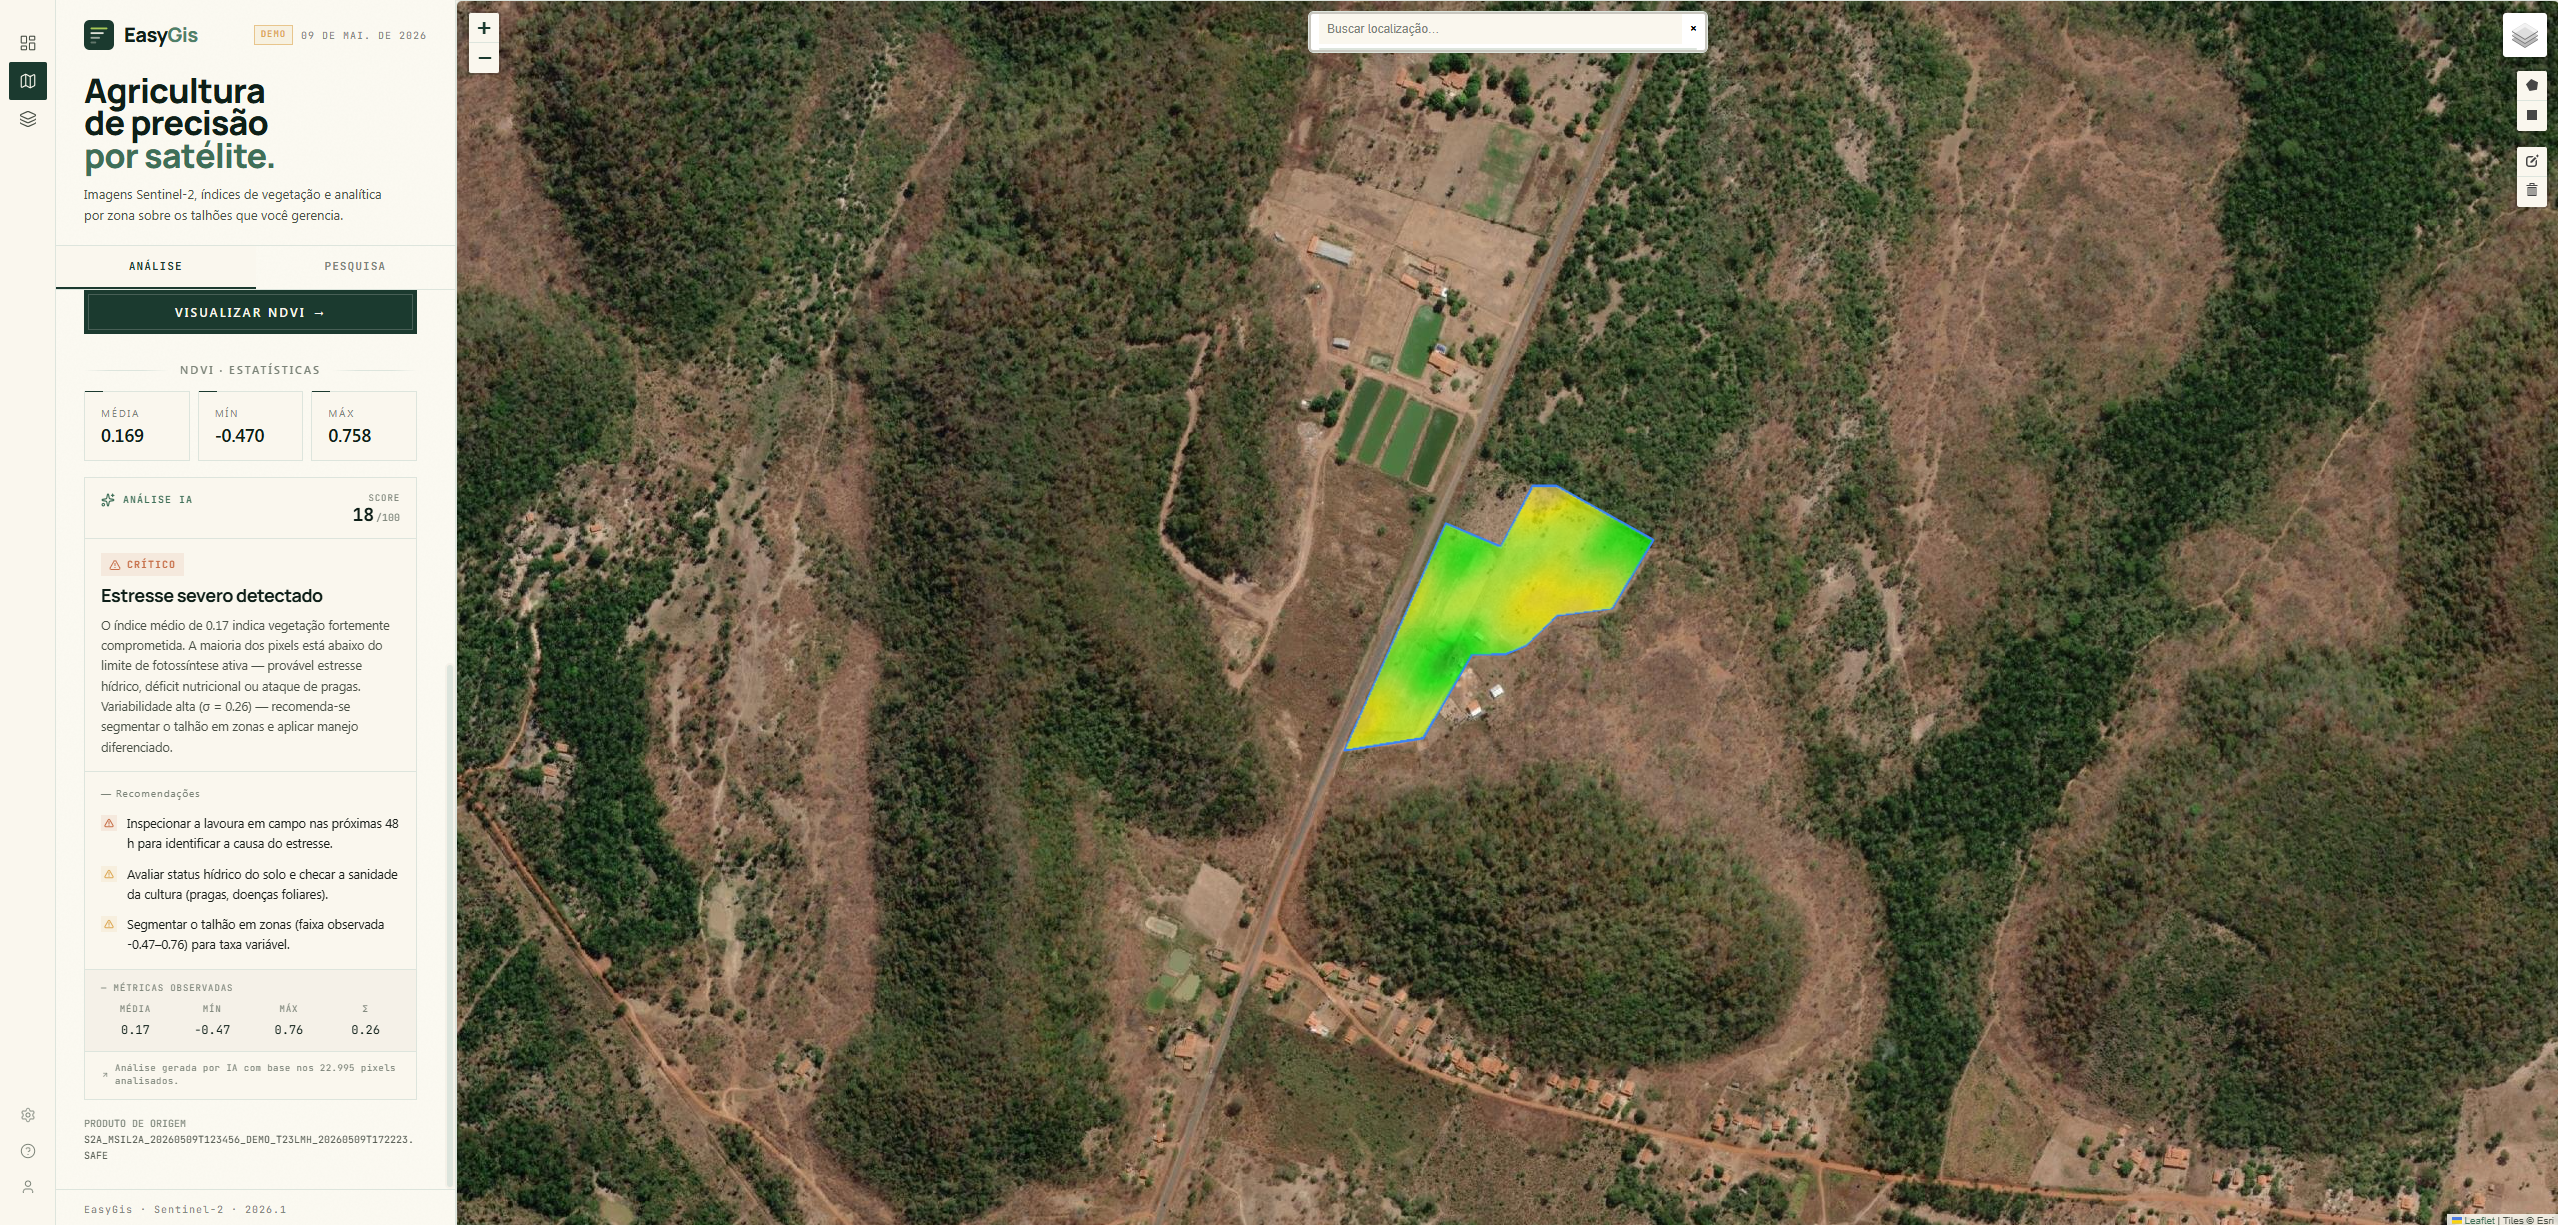
\includegraphics[width=\textwidth]{screenshots/MAN-03_ndvi-resultado}
\caption{Resultado de NDVI calculado sobre o talhão --- overlay colorido no mapa, estatísticas descritivas e histograma de distribuição no painel lateral.}
\end{figure}

\begin{infobox}[title={Como interpretar o NDVI}]
Se a média está \textbf{acima de 0,6}, a vegetação está saudável.\\
Entre \textbf{0,3 e 0,6}, em desenvolvimento ou estresse leve.\\
\textbf{Abaixo de 0,3}, área degradada, solo exposto ou estresse forte.
\end{infobox}

\subsection{Clicar em um ponto do mapa}

Depois do NDVI calculado, \textbf{clique em qualquer ponto} dentro do talhão. Aparecerá um popup classificando a saúde da vegetação naquele ponto exato:

\begin{itemize}
  \item \textcolor{errorred}{\textbf{Severo}} (NDVI $< 0{,}2$)
  \item \textcolor{warnyellow}{\textbf{Moderado}} ($0{,}2$ a $0{,}4$)
  \item \textbf{Leve} ($0{,}4$ a $0{,}6$)
  \item \textcolor{successgreen}{\textbf{Saudável}} ($\geq 0{,}6$)
\end{itemize}

\begin{figure}[H]
\centering
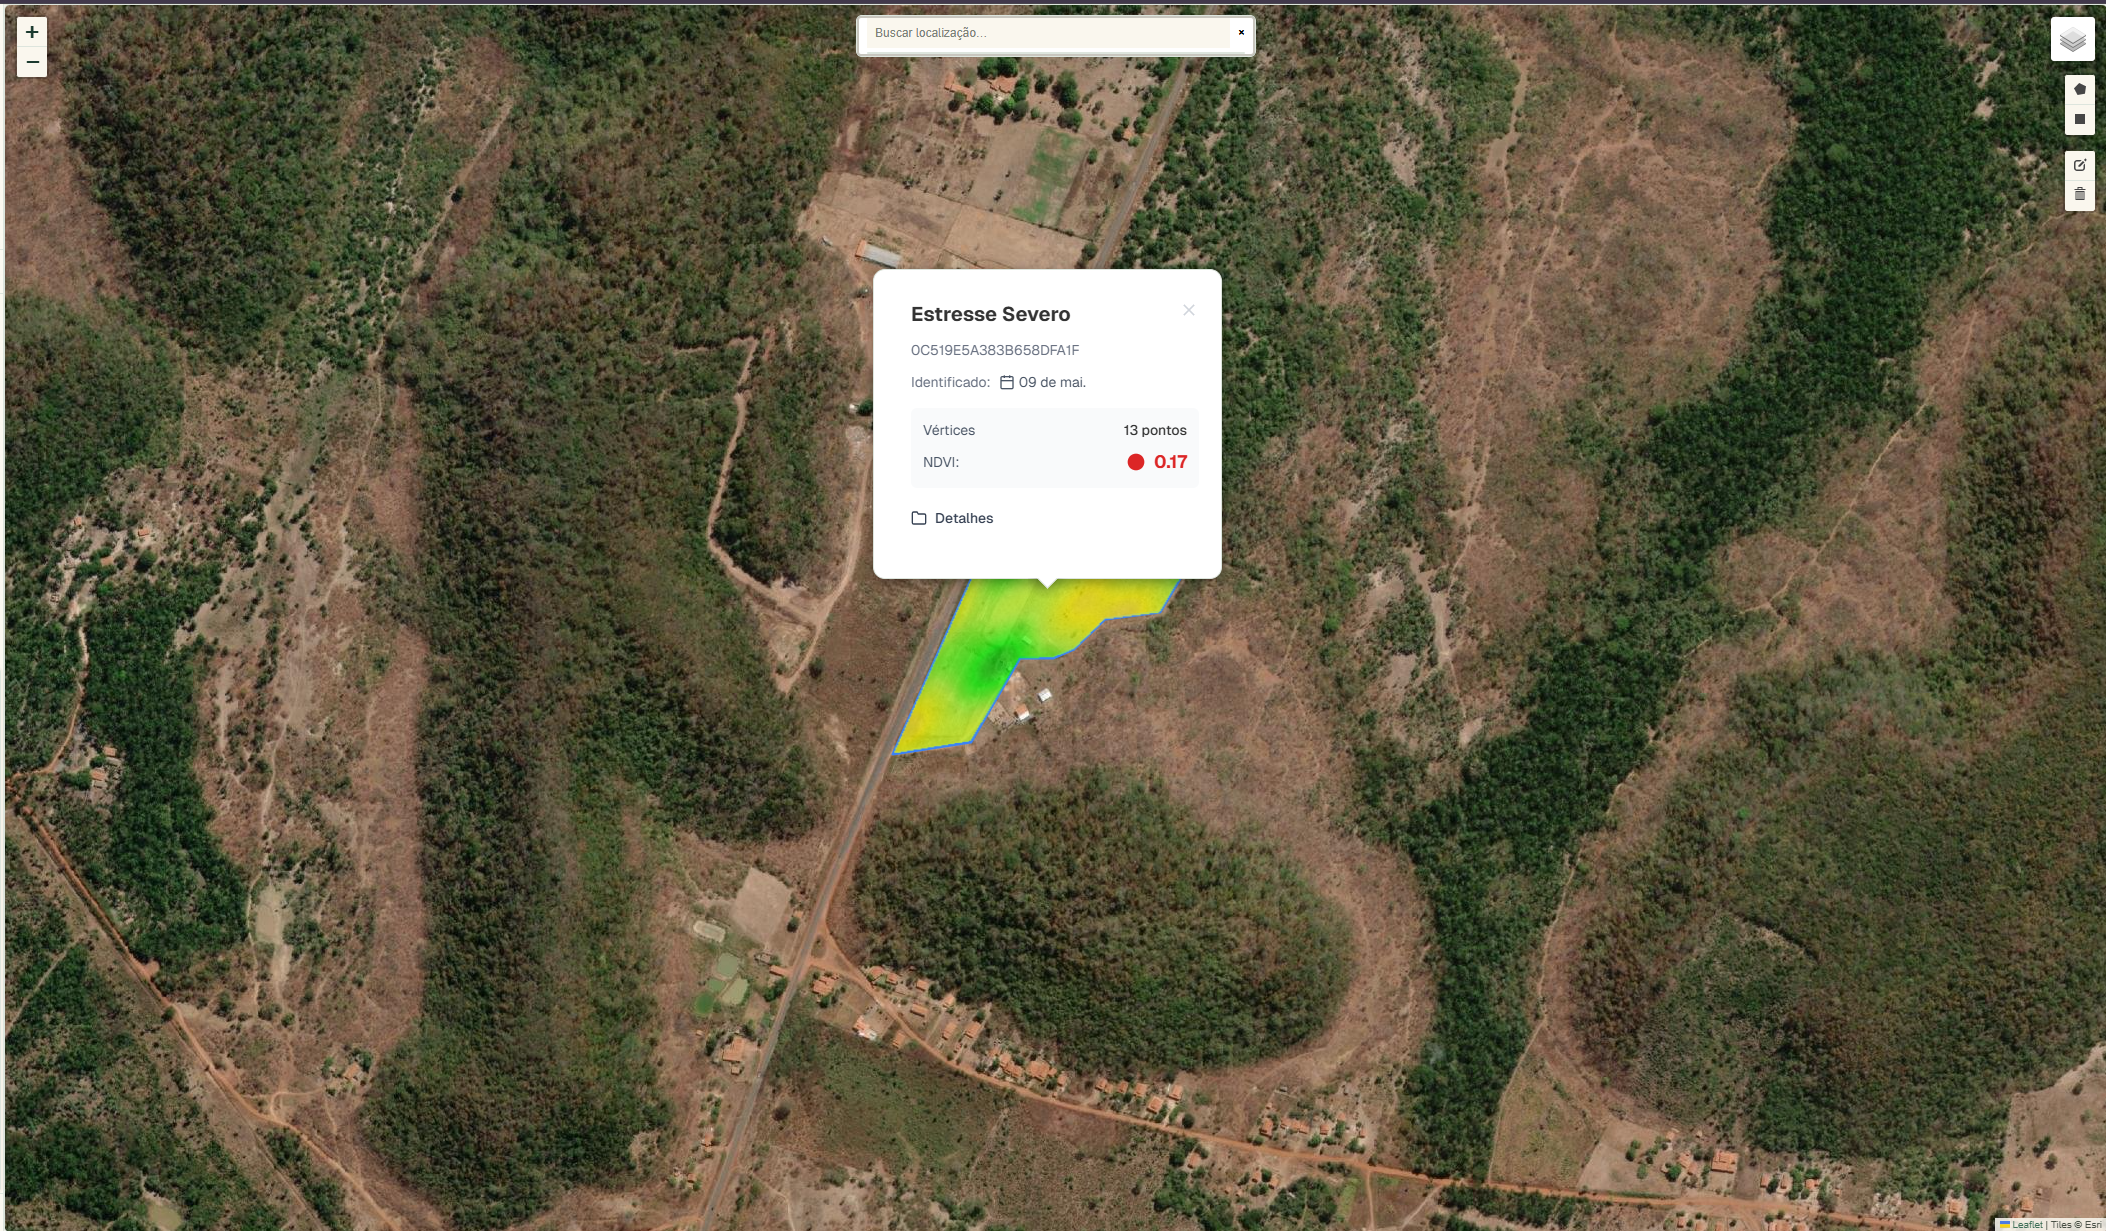
\includegraphics[width=\textwidth]{screenshots/MAN-04_popup-pixel}
\caption{Popup pixel-a-pixel ao clicar em um ponto do talhão --- mostra a classificação local de estresse vegetativo.}
\end{figure}

% ══════════════════════════════════════════════════════════════
\section{Outras análises disponíveis}
% ══════════════════════════════════════════════════════════════

\begin{table}[H]
\centering
\small
\rowcolors{2}{tabrow}{white}
\begin{tabularx}{\textwidth}{@{}lX@{}}
\toprule
\rowcolor{tabheader}\textcolor{white}{\textbf{Índice}} & \textcolor{white}{\textbf{Quando usar}}\\
\midrule
NDVI & Padrão para saúde geral da vegetação. Use sempre primeiro.\\
EVI & Quando o talhão tem vegetação muito densa (NDVI satura). Mais preciso em soja, milho maduros.\\
SAVI & Quando há muito solo exposto entre as plantas (lavoura jovem, café espaçado).\\
NDWI & Para ver umidade e estresse hídrico.\\
NDBI & Para identificar áreas construídas (não-agrícolas).\\
RGB & Foto colorida normal --- só visualizar o talhão.\\
FALSE\_COLOR & Composição em falsa-cor (vegetação aparece em vermelho). Padrão em fotointerpretação.\\
B01--B12 & Bandas individuais do satélite --- para usuários avançados que sabem o que cada banda revela.\\
\bottomrule
\end{tabularx}
\end{table}

\begin{figure}[H]
\centering
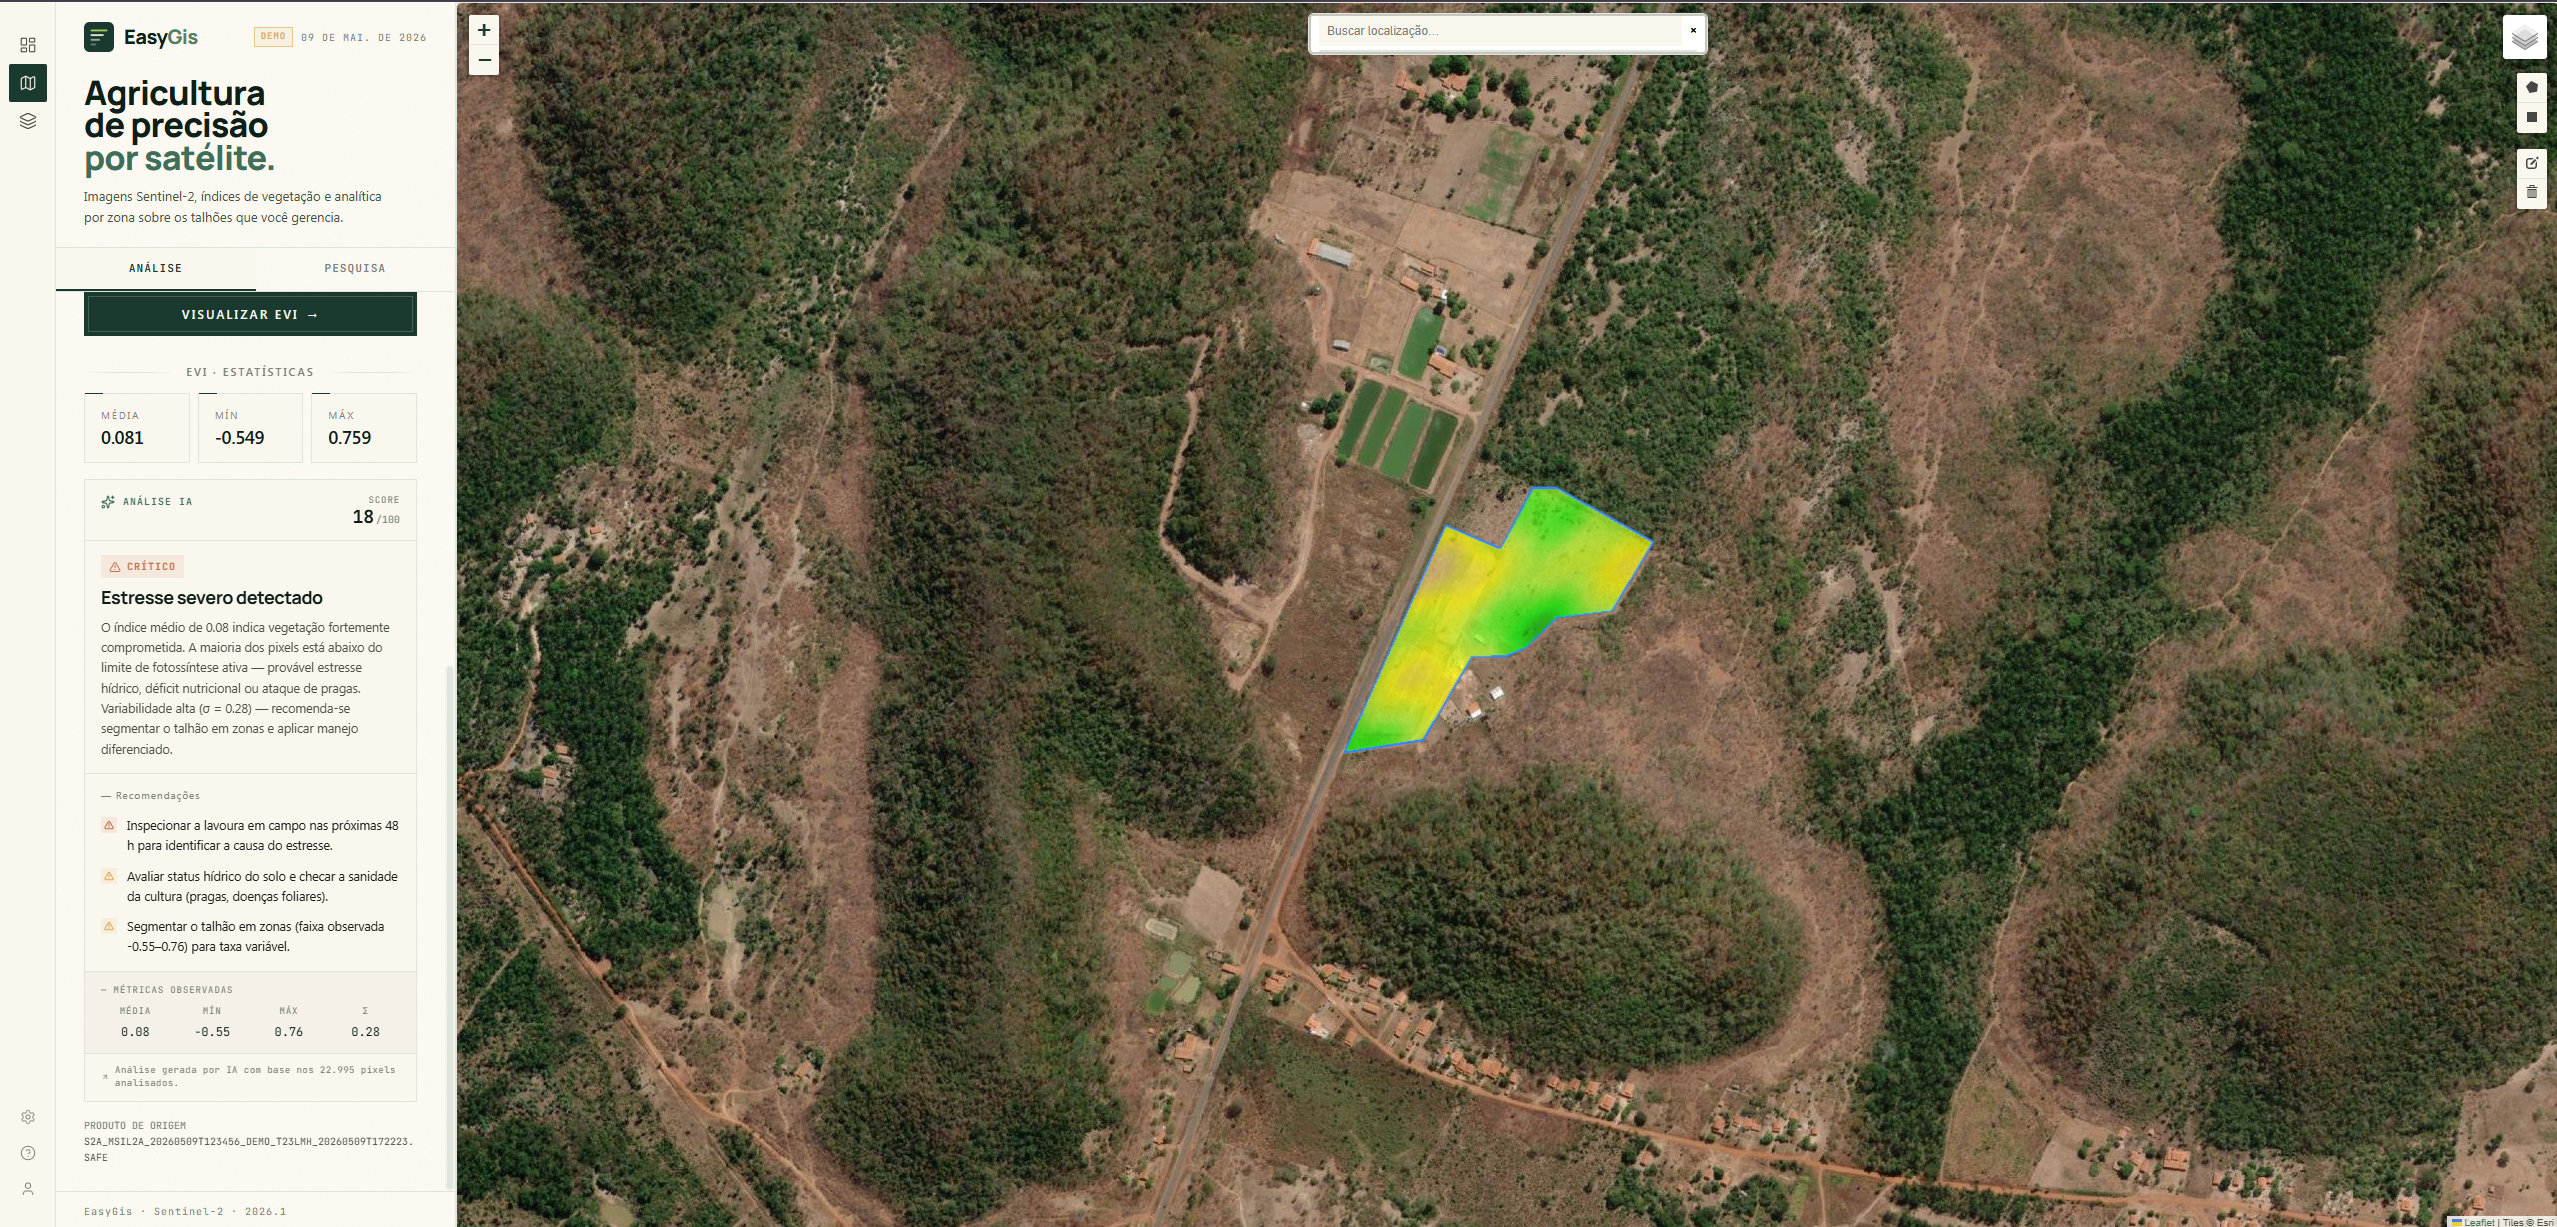
\includegraphics[width=\textwidth]{screenshots/MAN-05_evi-comparacao}
\caption{Resultado de EVI no mesmo talhão --- útil para comparar com o NDVI em vegetação densa, onde o NDVI satura.}
\end{figure}

\subsection{Suavização (opcional)}

Existe um botão \textbf{``Smooth''} que aplica um filtro para reduzir ruído na imagem. Use quando o talhão estiver muito ``granulado'' --- fica mais fácil ver padrões.

% ══════════════════════════════════════════════════════════════
\section{Visualização 3D}
% ══════════════════════════════════════════════════════════════

Após calcular um índice, ative o switch \textbf{``3D View''} no canto superior do mapa. A área se transforma em um relevo onde:

\begin{itemize}
  \item \textbf{Picos altos} = pixels com valor alto do índice (vegetação mais saudável)
  \item \textbf{Vales baixos} = valores baixos (estresse, solo exposto)
\end{itemize}

Você pode:

\begin{itemize}
  \item \textbf{Arrastar} com o mouse para girar
  \item \textbf{Rolar} para zoom
  \item \textbf{Clicar com botão direito + arrastar} para mover
\end{itemize}

Útil para enxergar variabilidade dentro do talhão de forma intuitiva.

\begin{figure}[H]
\centering
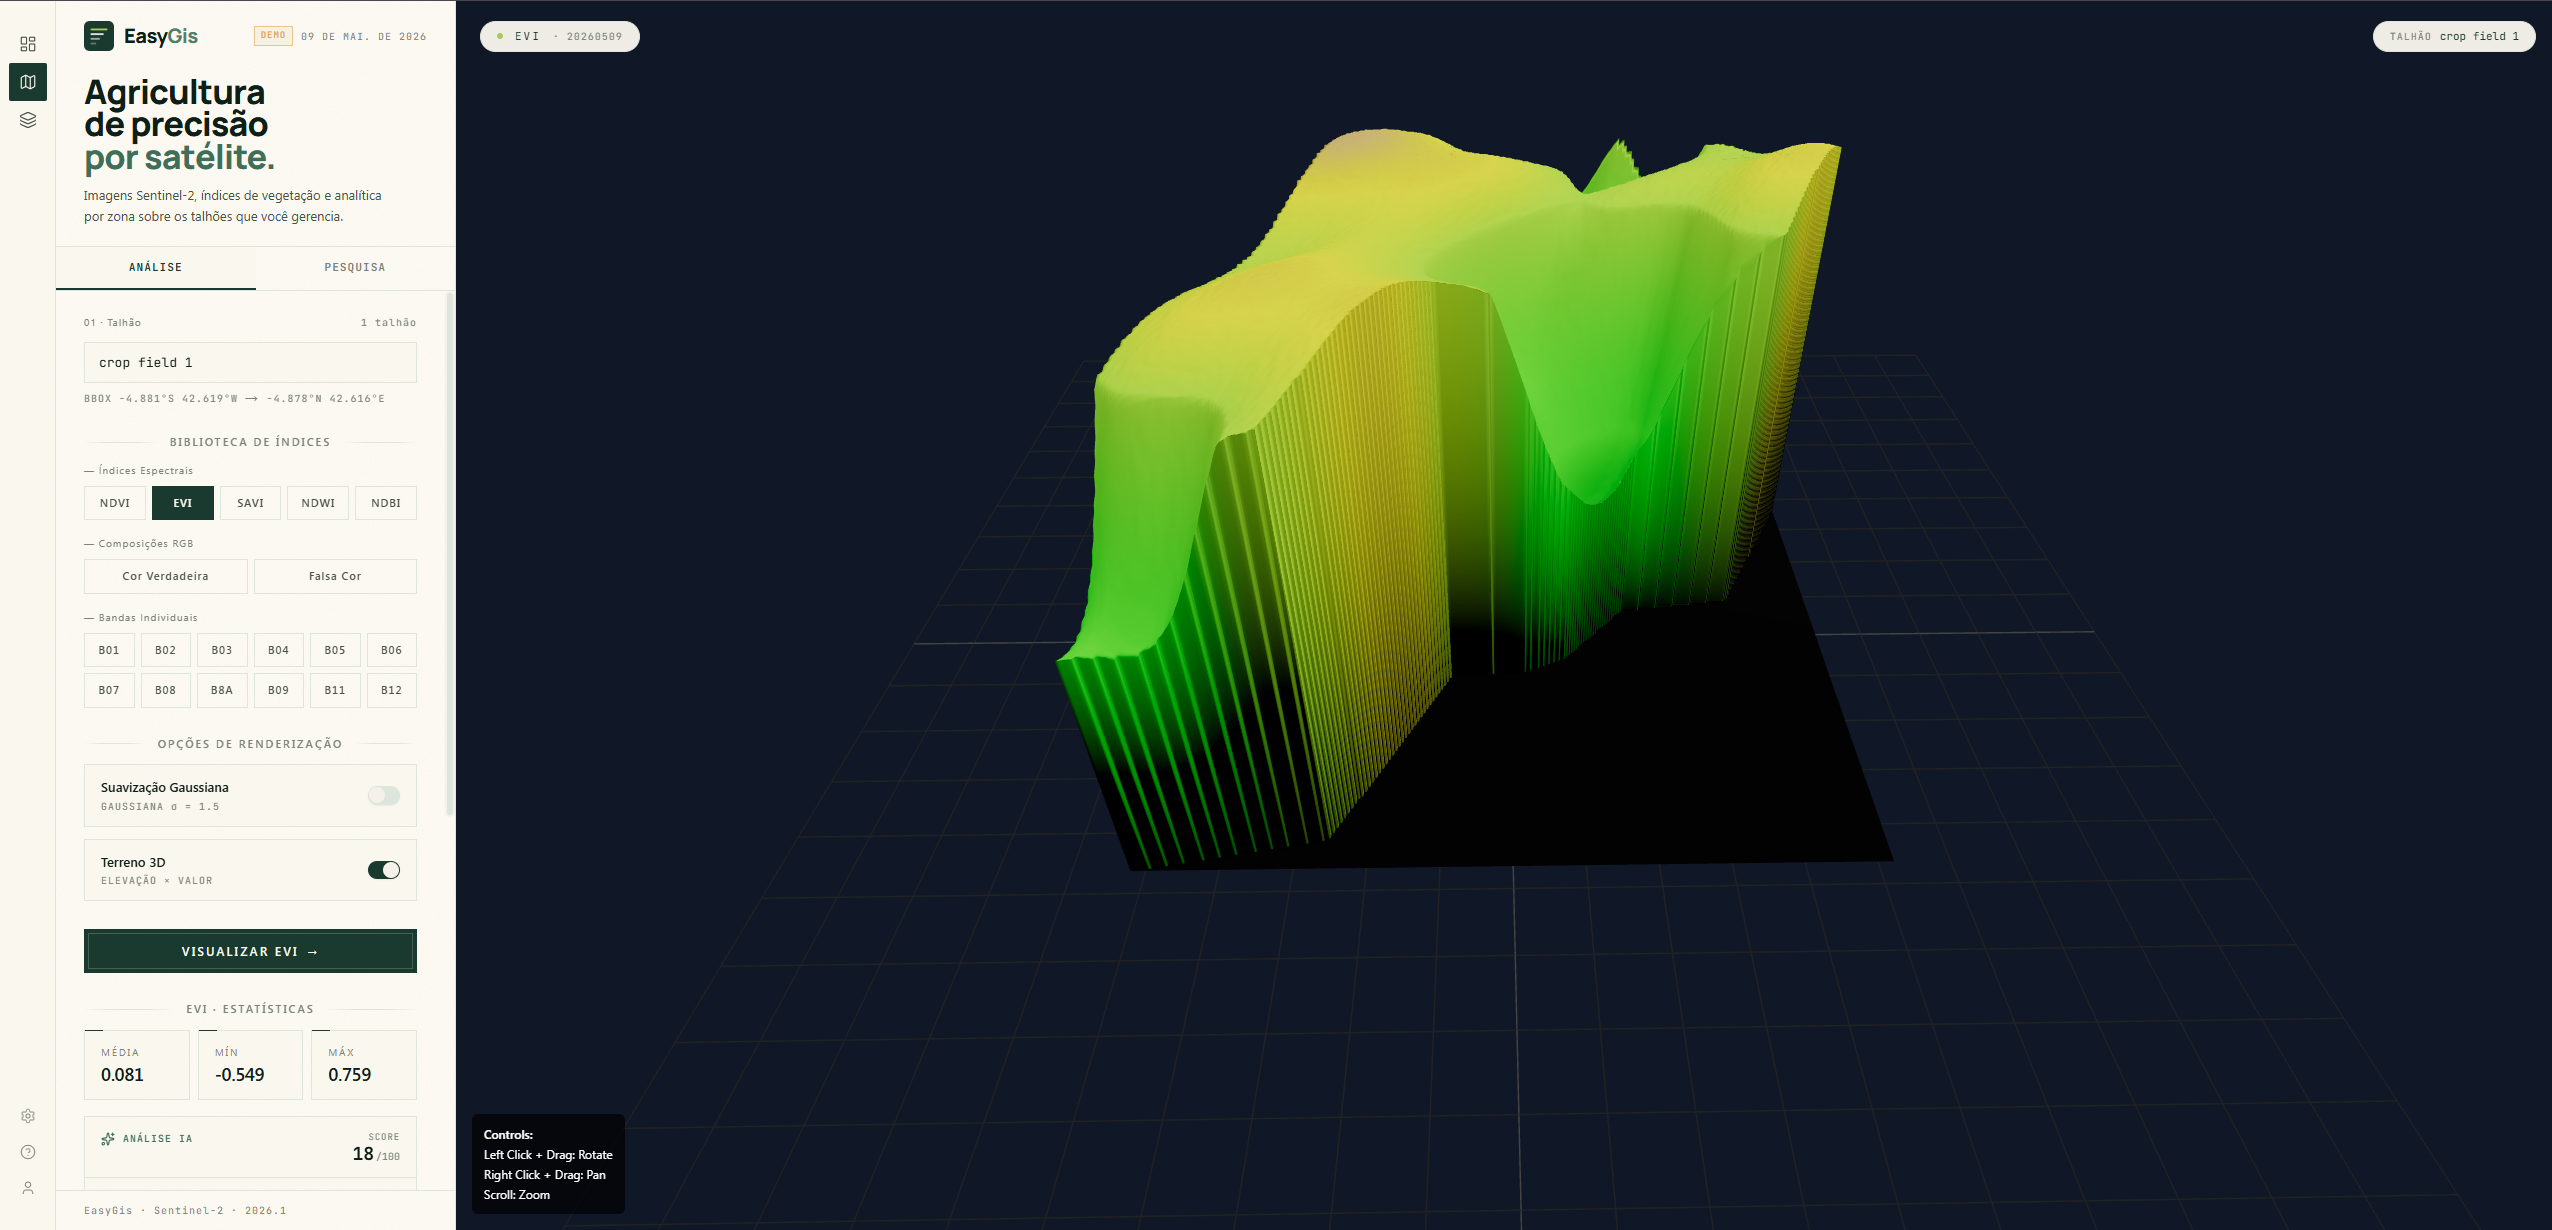
\includegraphics[width=\textwidth]{screenshots/MAN-06_3d-view}
\caption{Visualização 3D do índice como relevo --- picos altos indicam vegetação saudável, vales indicam estresse ou solo exposto.}
\end{figure}

% ══════════════════════════════════════════════════════════════
\section{Classificação de Culturas (página \texttt{/classification})}
% ══════════════════════════════════════════════════════════════

Para classificar o talhão em zonas, acesse o link \textbf{``Classification''} no topo do site (ou abra \url{http://localhost:3000/classification}).

\subsection{Três métodos disponíveis}

\subsubsection{1. Por Limiar (Threshold) --- recomendado para iniciantes}

Divide o talhão em 3 zonas usando NDVI:

\begin{itemize}
  \item \textcolor{errorred}{\textbf{Baixo Vigor}} (NDVI $< 0{,}3$) --- área que precisa de atenção urgente
  \item \textcolor{warnyellow}{\textbf{Médio Vigor}} ($0{,}3$ a $0{,}6$) --- área em desenvolvimento ou com estresse leve
  \item \textcolor{successgreen}{\textbf{Alto Vigor}} ($\geq 0{,}6$) --- área saudável
\end{itemize}

Cada zona vem com \textbf{\% e área em hectares} --- útil para planejar aplicação de insumos.

\begin{figure}[H]
\centering
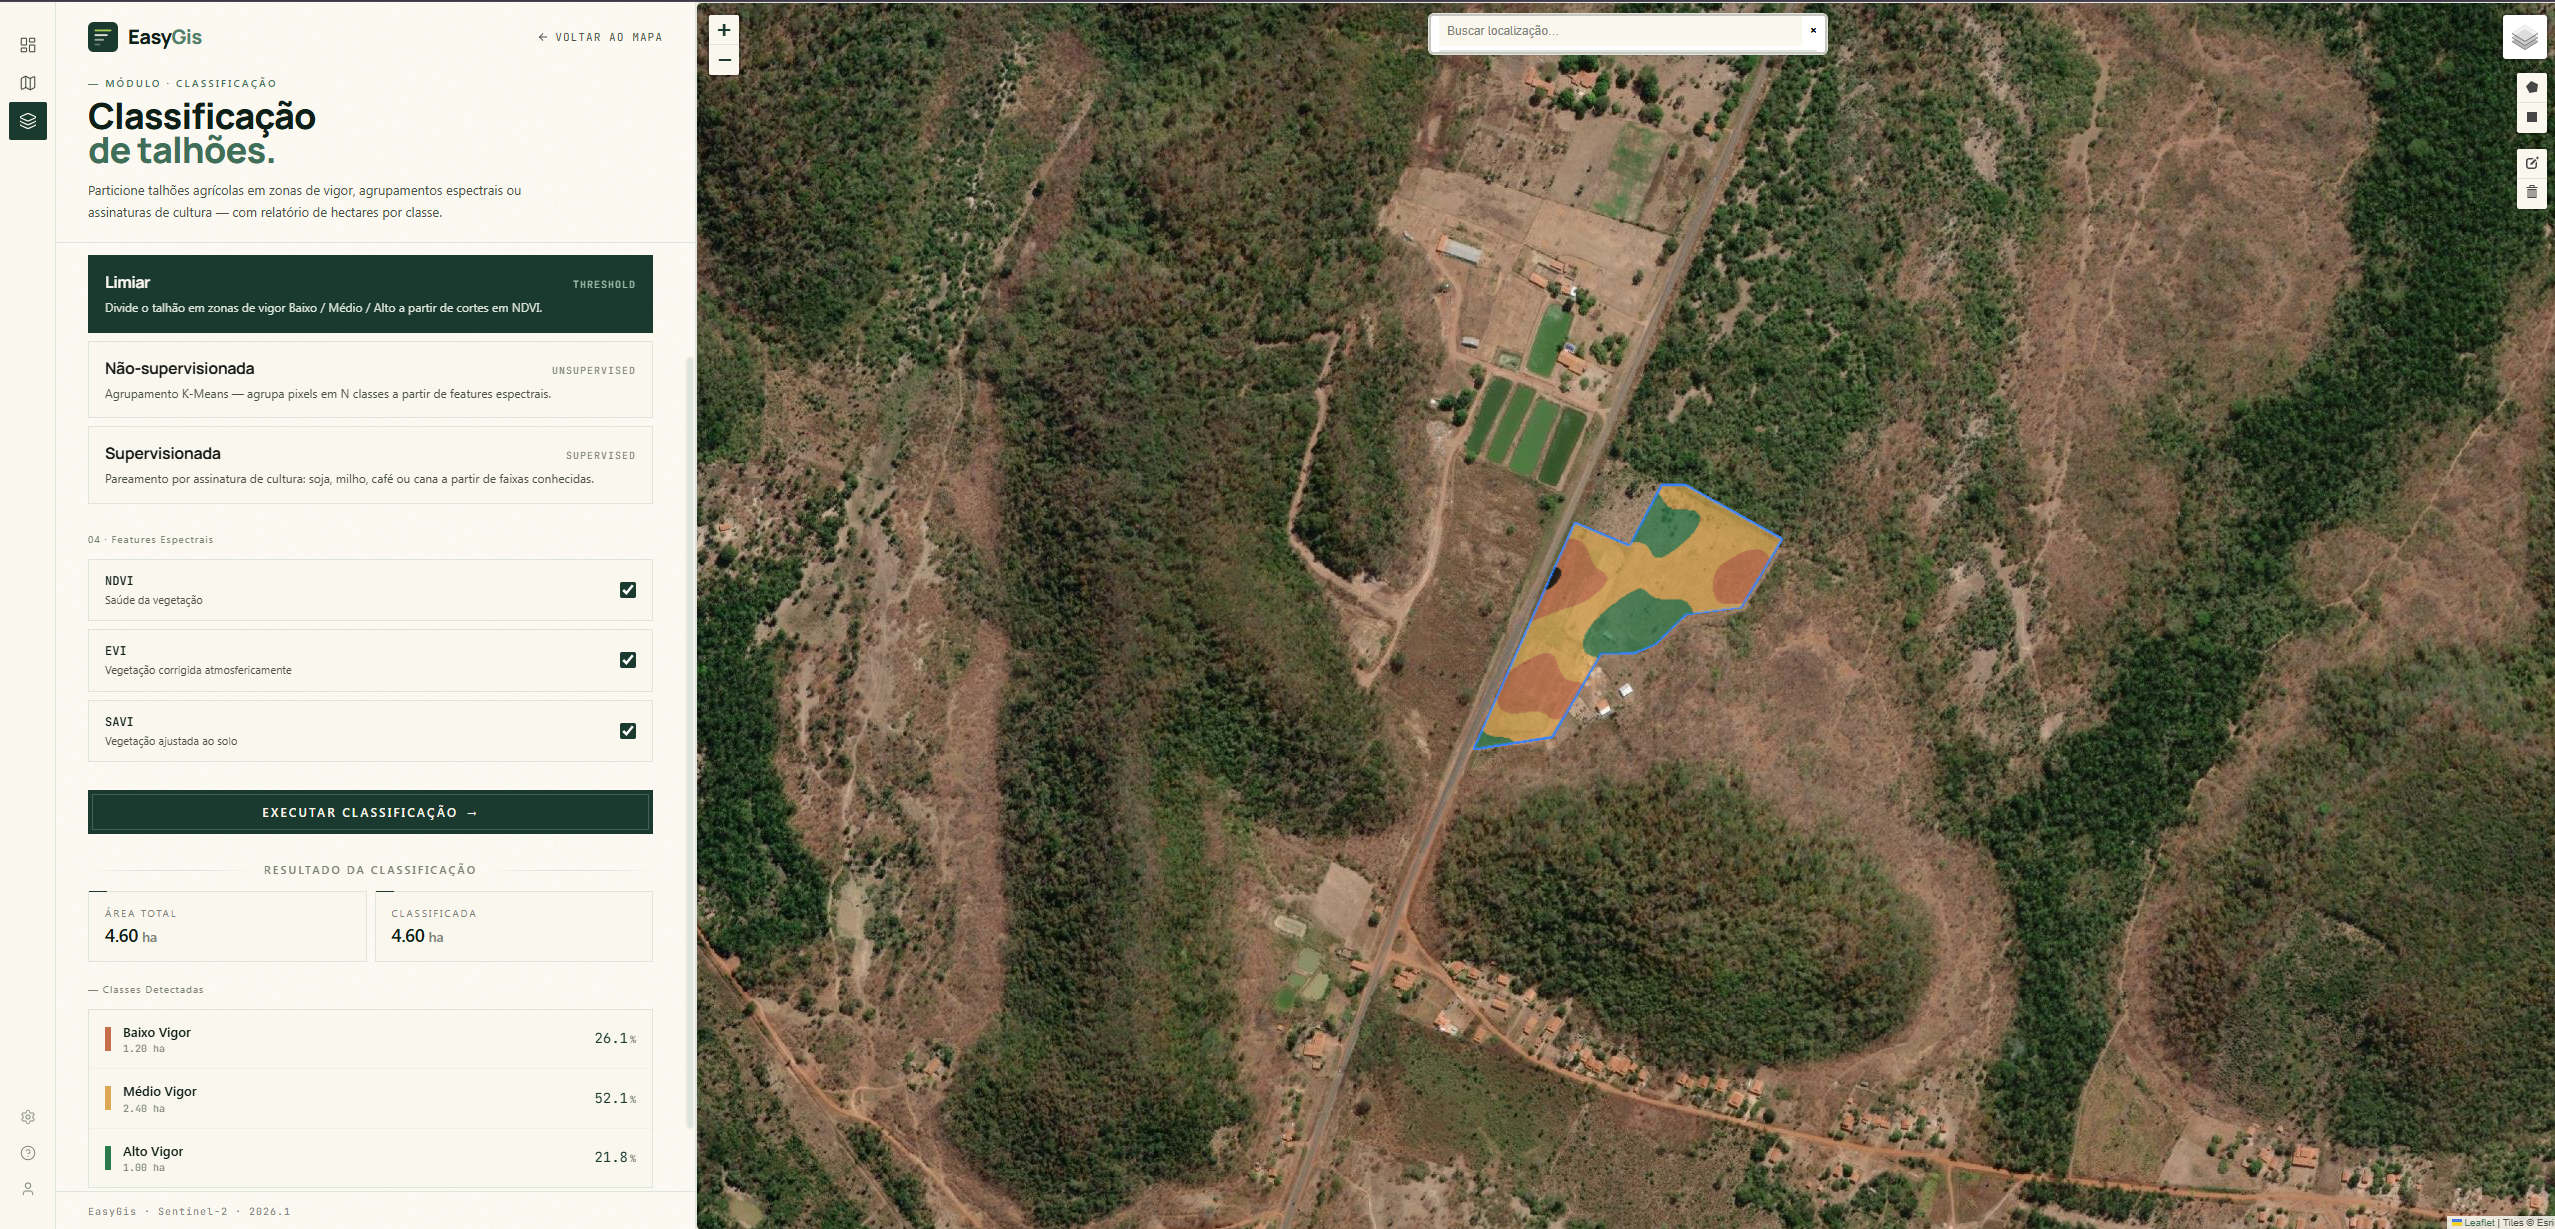
\includegraphics[width=\textwidth]{screenshots/MAN-08_threshold-vigor}
\caption{Classificação por Limiar (\textit{threshold}) --- 3 zonas de vigor com porcentagem e área em hectares.}
\end{figure}

\subsubsection{2. K-Means (Não-supervisionado) --- para análise exploratória}

Você escolhe quantas classes (de 2 a 6) e o sistema agrupa automaticamente. Bom para descobrir padrões que você não esperava.

\begin{figure}[H]
\centering
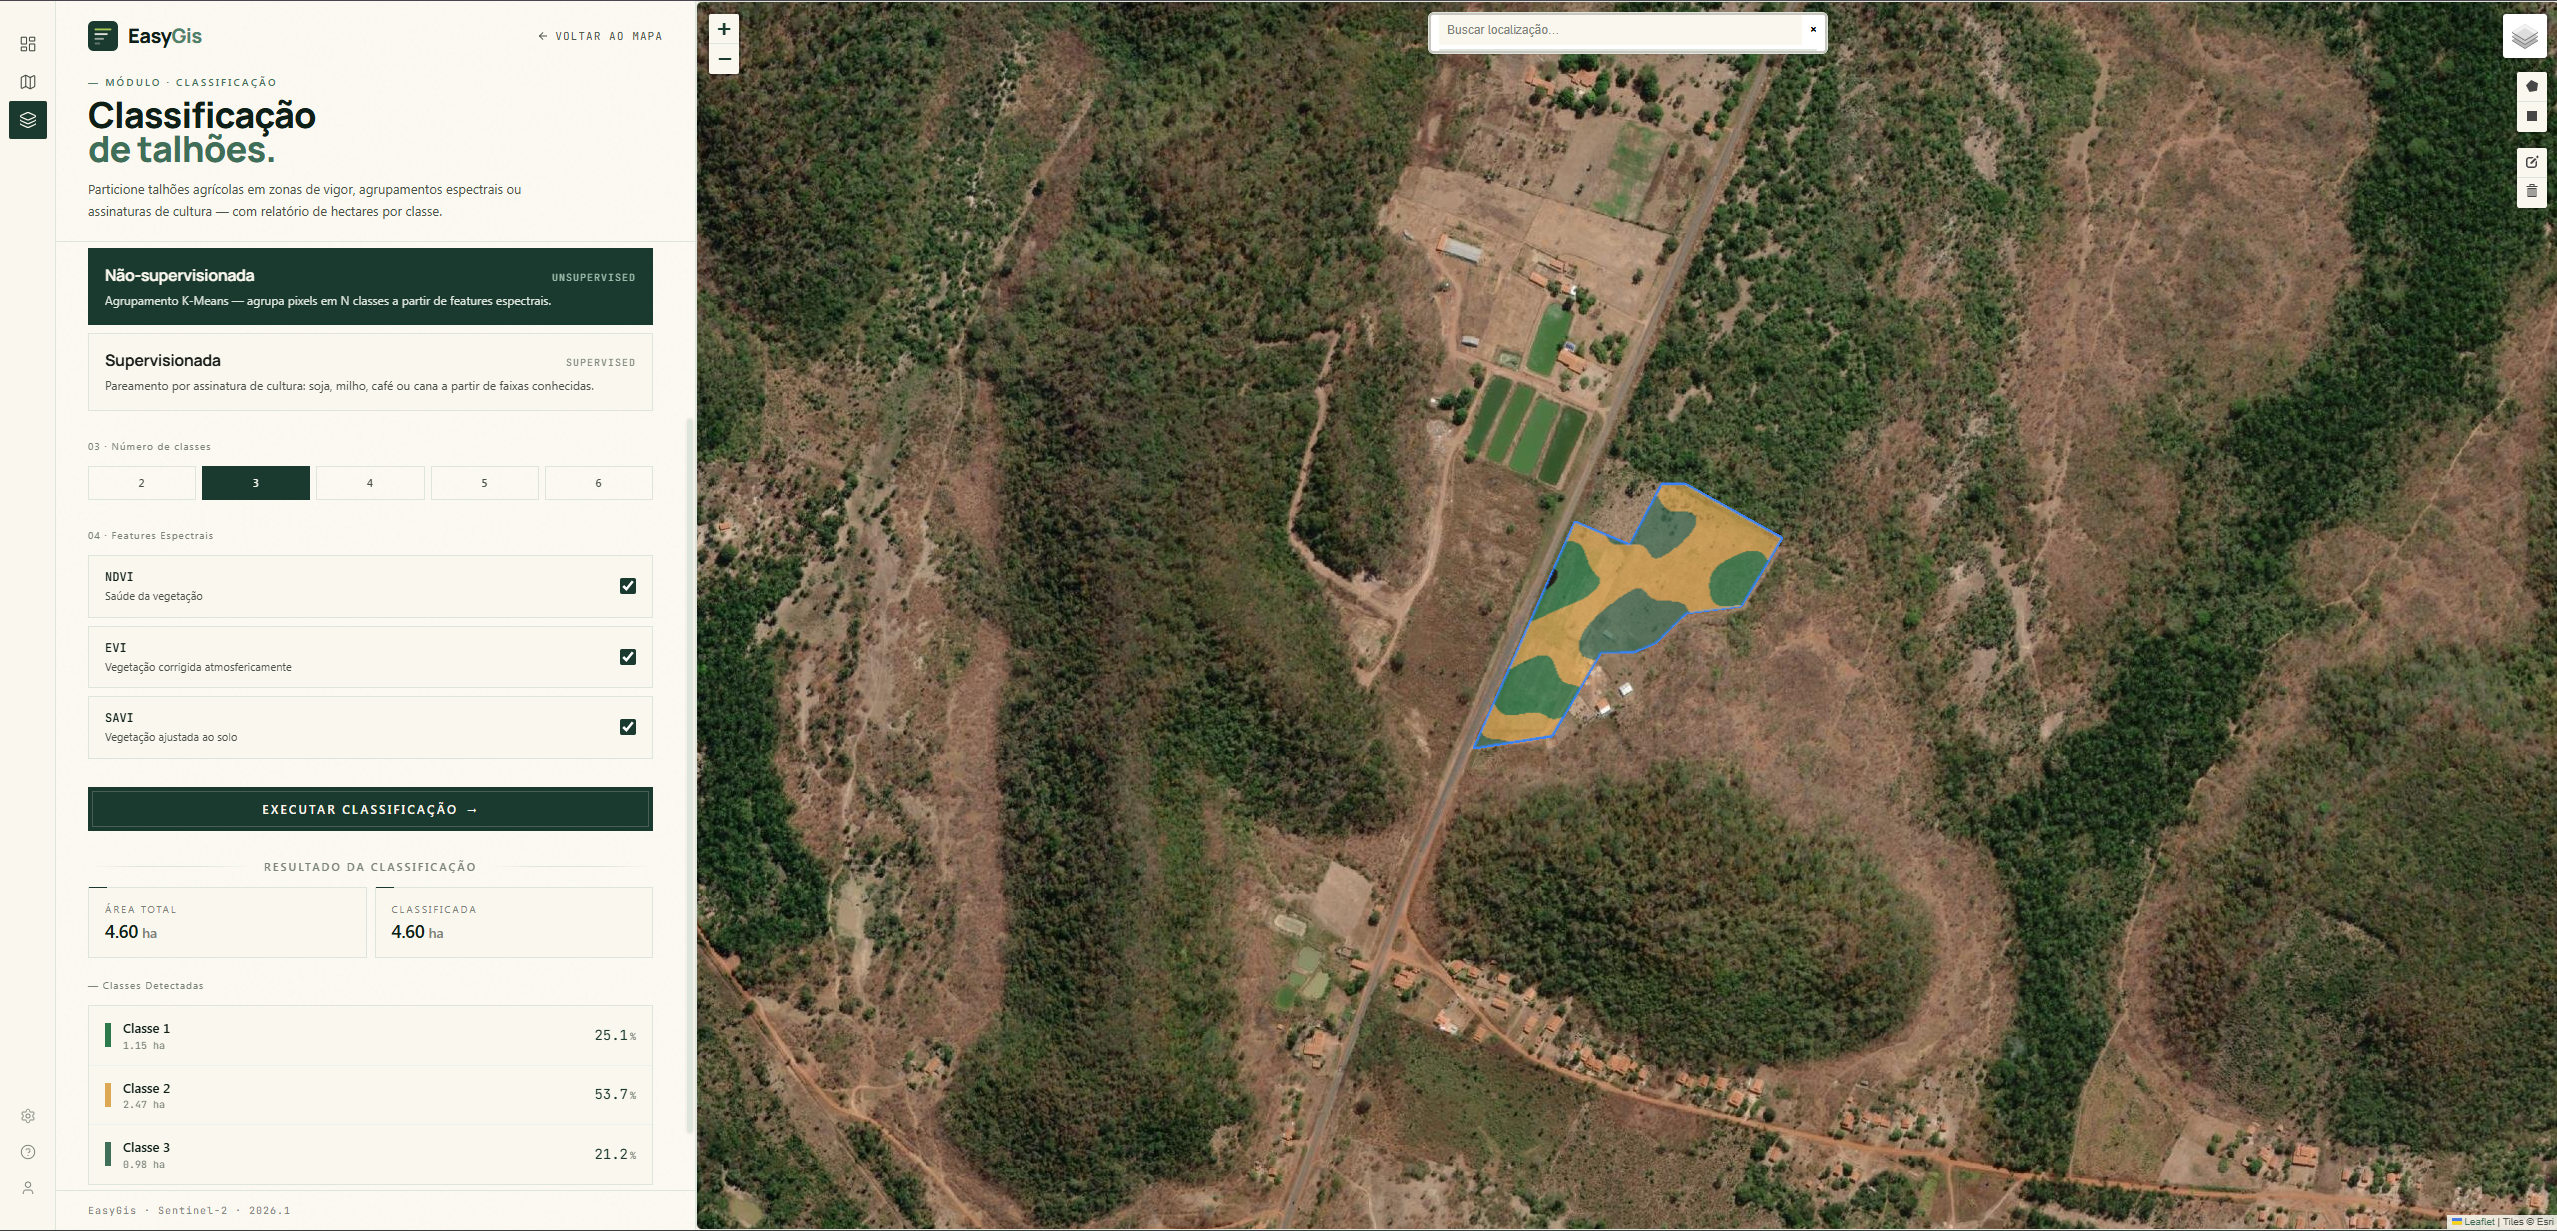
\includegraphics[width=\textwidth]{screenshots/MAN-07_classification}
\caption{Classificação K-Means com 3 classes --- agrupamento automático por similaridade espectral, ideal para encontrar zonas de manejo.}
\end{figure}

\subsubsection{3. Supervisionada (Simulada) --- demonstrativa}

Tenta identificar tipos de cultura (soja, milho, café, cana) com base em assinaturas espectrais conhecidas.

\subsection{Como rodar}

\begin{enumerate}
  \item Selecionar o talhão
  \item Escolher o método (recomendado: \textbf{Threshold} se estiver começando)
  \item Clicar em \textbf{``Classify''}
  \item Ver o resultado colorido no mapa + tabela com hectares de cada classe
\end{enumerate}

% ══════════════════════════════════════════════════════════════
\section{Laboratório de Experimentos (Aba ``Research'')}
% ══════════════════════════════════════════════════════════════

Para usuários avançados que querem aplicar técnicas de processamento de imagem. Funciona com a banda NIR (B08) por padrão. Você pode experimentar:

\begin{itemize}
  \item \textbf{Filtros} --- Suavizar imagem (Gaussiano, Mediana, Bilateral)
  \item \textbf{Detecção de Bordas} --- Achar limites entre tipos de cobertura (Sobel, Canny, Laplaciano)
  \item \textbf{Morfologia} --- Erosão, Dilatação, Abertura, Fechamento
  \item \textbf{Segmentação} --- Separar regiões (Limiar binário, Otsu, Adaptativo)
\end{itemize}

Em cada experimento, sliders permitem ajustar os parâmetros e ver o resultado em tempo real.

\begin{infobox}
Não é necessário entender todos os filtros --- eles servem como ferramenta de aprendizado e exploração.
\end{infobox}

% ══════════════════════════════════════════════════════════════
\section{Perguntas Frequentes}
% ══════════════════════════════════════════════════════════════

\subsection*{``Por que demora tanto para calcular?''}

Porque o sistema lê arquivos de satélite com centenas de megabytes e faz o recorte na hora. Para um talhão típico (até 100 ha), espere de 5 a 30 segundos. Talhões muito grandes podem levar mais.

\subsection*{``Os meus talhões somem quando recarrego a página.''}

Sim, no MVP atual o sistema não salva o estado entre sessões. Os talhões importados via KML são lidos do disco toda vez (em \texttt{data/KML Fields/}), então esses ficam. Apenas os desenhados manualmente no mapa são perdidos.

\subsection*{``Como adiciono um novo talhão?''}

\textbf{Opção 1 --- KML (recomendado):} No Google Earth, desenhe um polígono e exporte como \texttt{.kml}. Coloque o arquivo em \texttt{data/KML Fields/} e recarregue a página --- ele aparecerá no dropdown.

\textbf{Opção 2 --- Desenhar no mapa:} Use os ícones de polígono/retângulo no canto esquerdo do mapa. O talhão aparece imediatamente para análise (mas não fica salvo após recarregar).

\subsection*{``Como adiciono uma nova imagem de satélite?''}

Baixe um produto Sentinel-2 Level-2A do \href{https://browser.dataspace.copernicus.eu/}{Copernicus Open Access Hub} e descompacte o \texttt{.SAFE} em \texttt{data/products/}. O sistema usa automaticamente a imagem mais recente.

\subsection*{``Apareceu uma mensagem de erro vermelha. O que faço?''}

A maioria dos erros está descrita na própria mensagem. Os mais comuns:

\begin{itemize}
  \item \textbf{``No products found''} --- você esqueceu de colocar a imagem \texttt{.SAFE} em \texttt{data/products/}
  \item \textbf{``Field not found''} --- o talhão não foi carregado; verifique se o arquivo \texttt{.kml} está em \texttt{data/KML Fields/}
  \item \textbf{``Polygon outside image bounds''} --- o talhão está em uma região não coberta pela imagem; baixe outra imagem da área correta
\end{itemize}

Se o erro persistir, peça ajuda ao administrador.

\subsection*{``O 3D está travando o navegador.''}

Use a aba ``Analytics'' sem ativar o 3D. A renderização 3D exige GPU e pode pesar em máquinas mais antigas. Talhões muito grandes geram mais polígonos --- tente um talhão menor para testar.

% ══════════════════════════════════════════════════════════════
\section{Glossário}
% ══════════════════════════════════════════════════════════════

\renewcommand{\arraystretch}{1.3}
\begin{table}[H]
\centering
\small
\rowcolors{2}{tabrow}{white}
\begin{tabularx}{\textwidth}{@{}lX@{}}
\toprule
\rowcolor{tabheader}\textcolor{white}{\textbf{Termo}} & \textcolor{white}{\textbf{Significado simples}}\\
\midrule
NDVI / EVI / SAVI & ``Termômetros'' da saúde da plantação. Calculados a partir de bandas do satélite.\\
Banda & Cada cor que o satélite enxerga (incluindo cores invisíveis ao olho humano, como infravermelho).\\
Sentinel-2 & Satélite gratuito da Europa que fotografa o Brasil a cada 5 dias com resolução de 10 metros.\\
Talhão & Área de cultivo definida por seus limites geográficos.\\
KML & Formato de arquivo do Google Earth para guardar polígonos.\\
Hectare (ha) & 10\,000 m\textsuperscript{2} (um quadrado de 100 $\times$ 100 metros).\\
\bottomrule
\end{tabularx}
\end{table}

\vfill
\begin{center}
\small\textit{Em caso de dúvida, problema ou sugestão, contate a equipe de desenvolvimento\\ou consulte os documentos técnicos em \texttt{docs/}.}
\end{center}

\end{document}
